\PassOptionsToPackage{unicode}{hyperref}
\PassOptionsToPackage{hyphens}{url}
%
\documentclass[12pt, a4paper]{article}
\usepackage[a4paper,margin=1in]{geometry}
\setlength\parindent{0pt}
\usepackage{mathptmx}
\usepackage{amsmath, amssymb}
\usepackage[T1]{fontenc}
\usepackage[utf8]{inputenc}
\usepackage{textcomp}
\usepackage[colorlinks=true, urlcolor=blue, citecolor=black, linkcolor=black]{hyperref}
\usepackage{xcolor}
\usepackage{siunitx}
\usepackage{graphicx}
\graphicspath{ {./images/} }
\usepackage{float}

\author{Davide Cremonini, Artificial Intelligence, 0001137778
\\Alessia Crimaldi, Artificial Intelligence, 0001145505
\\Fabio Giordana, Artificial Intelligence, 0001145924
\\Gabriele Nanni, Artificial Intelligence, 0001146107}
\date{}
\title{Social Network Analysis of Twitter Bots}

\begin{document}
\maketitle


% Report in PDF format of at most 5000 words (also after revisions) — approximately, these correspond to 30k characters and 9–10 pages.

% CHECKLIST!!!!!!

% [ ]  It is clear how many networks you are going to analyse and their shape (monomodal, bipartite, etc.).

% [ ]  For each network in the study, it is clear what are the nodes and what are the edges (when there exists an edge between nodes) and whether these are oriented or not.

% [ ]  You apply a wide-enough range and number of measures to describe the phenomena you want to study (measures include centrality, groups, clustering, redundancy, equivalences, homophily, small-worldness, scale freedom, cohesion, connectedness, compactness, triad census, core-periphery, etc.).

% [ ]  For each measure, you explain why you apply it (what phenomenon you investigate with it) and what semantics the measure has for your network (e.g., on a transport network, you apply betweenness centrality to find its most important junctions, since it measures the extent to which a node lies on paths between other nodes).

% [ ]  The effort behind the study is appropriate for the number of students behind the project. Suggestion: projects can consider applying the same study design on different networks, to compare these (qualitatively and/or quantitatively) through the results of the same array of measures.	


\section{Introduction}
	\label{introduction}
	% The context includes: the general field (e.g., literature, history, archaeology, tourism, biology, forensics, religious studies); the specific application (e.g., literary analysis, quantitative history, genetics, virology, forensics intelligence, tourism planning, biblical quantitative studies).
	In the current historical moment, the widespread diffusion of AI systems designed to simulate human behaviour is increasingly evident. Our project aims to evaluate the effectiveness of these systems in the context of bot detection on Twitter, seeking to identify behavioural patterns that differentiate automated users (aka \textit{bots}) from human ones. To this end, we make use of Social Network Analysis techniques.


\section{Problem and Motivation}
	\label{problem-and-motivation}
	% What are the problems you want to address? Why are those problems important (impact, theoretical and/or practical needs, etc.)? What are the main contributions of the project?
    Nowadays it is clear the impact of social medias in the everyday life of people. These applications are not only a way to interact with friends or observe celebrities, but they are becoming one of the most impacting form of information for all generations, from middle-aged demographics to young adults, interacting also with children most of the population extracts their knowledge through social media. The creation of automated accounts on these platforms can impact the perception of people spreading false information or polarising content, causing a clash between two sides not willing to discuss and find a middle ground. Bots can also post and interact with other accounts, show a different distribution of opinions with respect to the real one, causing public opinion to be shifted and inducing entities like companies or public organisations to move in certain directions because of the feedback given by them.\\
    For these reasons we wanted to observe the behaviour of bots and human accounts to find a way to detect patterns that characterise one's relations. The focus of this project are the relations between the accounts, in the form of the "follow" action. This action is performed from one account to another, signalling that the user is interested in receiving updates on the interactions of that account, and it can be reciprocated.


\section{Datasets}
	\label{datasets}
	% How did you gather the data? Did you digitise it? How? Is the material publicly available? What tools did you use 1) to handle (store, manipulate) the data and 2) to compute measures on the data?
	We conducted our analysis using the TwiBot-22 dataset \cite{twibot22}, which is publicly available on GitHub\footnote{\href{https://github.com/LuoUndergradXJTU/TwiBot-22}{https://github.com/LuoUndergradXJTU/TwiBot-22}}.\\
	TwiBot-22 is a comprehensive, graph-based benchmark for Twitter bot detection, featuring the largest dataset available up to date. It offers a diverse range of entities and relationships within the Twitter network, and boasts significantly improved annotation quality compared to previous datasets.\\
	Given the extremely large size of the dataset it is impossible to work with the full dataset with our resources. For this reason preprocessing has been used to elaborate the dataset more efficiently.
    \subsection{Preprocessing}
    	The two files we focus on are tweets and edges. The preprocessing is needed to extract the relation \textit{follower-following} for every user to build the network and to obtain the number of tweets of each user.	 Therefore, we create chunks for edges and for tweets that is possible to store in the avaliable RAMs.\\
        After this technical solution to be able to work with all data we proceed to creating the communities. The communities are sub-networks of people who used the same hashtag in their tweets. They will be used to check if the patterns found in the network are robust to network changes or are network-specific. To test the robustness of the patterns we divided the subnetworks into different categories (large, medium and small communities) to test the results on different scales.
	\subsection{Adopted tools}
		The Python libraries used in this project are:
        \begin{itemize}
            \item the \textit{Polars} library and the \textit{ijson} parser for the manipulation of the dataset.
            \item the \textit{NetworkX} \cite{hagberg2008} and \textit{NetworKit} \cite{staudt2016} libraries to create the network and to calculate the measures on it.
            \item the \textit{seaborn}, \textit{SciPy} and \textit{scikit-learn} libraries to search for possible patterns in the bots/humans behaviour.
        \end{itemize}
	\subsection{Analyzed networks}
    	As discussed above, we divided subnetworks into three classes, based on the number of nodes (i.e. users) they contain: small networks have less than 1000 nodes, medium-sized have between 1000 and 10000, and large have more than 10000. Among each class we chose to focus on communities which may present more polarising opinions as they discussed hot topics at the time of the dataset creation.
    	\begin{itemize}
			\item Large $\rightarrow$ Ukraine, Ai, Covid
			\item Medium $\rightarrow$ Nato, Deeplearning, Nftcommunity
			\item Small $\rightarrow$ Ruleoflaw, Feminist, Agenda2030
		\end{itemize}
		An interactive graphical version of the analyzed subnetworks is available \href{https://alessiacrimaldi.github.io/sna_project/}{here}. Figure~\ref{fig:feminist_subnetwork} illustrates the feminist subnetwork, where node size indicates the number of tweets authored by each account. Nodes representing bots are colored in red, while human users are shown in green.
		\begin{figure}[H]
    		\centering
    		\includegraphics[width=\textwidth]{feminist_subnetwork.png}
    		\caption{Feminist subnetwork {\footnotesize (\href{https://alessiacrimaldi.github.io/sna_project/results/subnetworks/feminist/feminist_network}{link})}}
    		\label{fig:feminist_subnetwork}
		\end{figure}
		

\section{Validity and Reliability}
	\label{validity-and-reliability-not-needed-for-the-project-proposal}
	% How closely does the model of your dataset represent reality (validity)? How does the way you treat the data affect the reproducibility of the study (reliability)?
	As discussed in its official paper \cite{twibot22}, the TwiBot-22 dataset was created trying to address and mitigate known problems of previous datasets, such as poor annotation quality and low dataset scale. This led to the construction of a large social graph with real world tweets, relationships between entities and metadata. This design allows the results to be statistically relevant, and it accurately reflects Twitter’s social dynamics. Moreover, the dataset benefits from a strong annotation pipeline, which guarantees reliability and consistency, and reproducibility for a wide range of bot detection and behaviour analysis studies. It is also easily accessible and freely available.\\
    In our work, we exploited the dataset focusing only on \textit{follower-following} relationships between users. Additionally, we experimented with applying the same analytical measures to the full graph and subgraphs based on shared hashtags, in order to introduce a topical dimension to our analysis. This approach maintains the validity of the dataset, as both the follower links and the shared hashtag activity represent authentic user behaviours and capture meaningful patterns within Twitter’s social structure. Our results are also fully reproducible and reliable, as we provide a detailed description of the preprocessing pipeline used to tailor the dataset to our specific research goals.


\section{Measures and Results}
	\label{measures}
	% What measures did you apply (brief explanation of how they work)? How do they relate to the intent of the study? Why are they relevant? What is the connection among the gathered data, the applied measures, and the properties found?
	The experiments were all conducted on an NVIDIA GeForce RTX 3090 GPU (24GB VRAM).
	\subsection{Measuring the Network}
    	One of the core assumptions which guided us in our study was the idea that bots show different behaviour when it comes to forming follower-following relationships with other users: specifically we expect bots to form less homogeneous connections, more based on random choices with respect to humans. As a consequence, we expect the presence of bots to have an effect on the overall network.\\
    	As a preliminary examination, to confirm our suppositions on bot behaviour, we decided to conduct some measurements on the entire network. Given the size of the dataset, the feasibility of some of these measures was conditioned by the computational limitations.\\
    	To highlight the effects of bots on the network, we created three main versions of the original follower-followed graph: 
        \begin{itemize}
            \item original graph, with 693.761 users
            \item human nodes graph, obtained by considering only human users, having 612.329 nodes
            \item human-human edges graph, obtained by considering only human users connected only to other human users, with 589.924 nodes.
        \end{itemize}
        A key difference between the second and third subgraphs is that the latter excludes all those human users who were only followed or were followed by bots, a total of 22.405 users.\\
        We then proceeded by analysing the number of components present in each of these graphs, discovering that there seems to be only one main large component which constitutes most of the graph, both in the first and third cases. As expected, the second subgraph presented a high number of isolated users.\\
        The next step was verifying the scale-free nature of these networks. To do so, we computed the degree centrality of all nodes and tested their distribution, fitting a power law and observing the results. The results were positive, since all three of them fitted perfectly in a power-law distribution, having \(2<\alpha<3\). This is a further confirmation of the resilience of these types of networks to disruption and scale change, which should prove helpful for sub-sampling in the next steps.\\
        Finally, we decided to test our hypothesis on bot behaviour by computing density and clustering coefficient on the networks with and without them, and we found the results shown in Table~\ref{tab:network_measures}.
        \begin{table}[h]
            \centering
            \begin{tabular}{|c|c|c|}
            	\hline
            	\textbf{Network}   &  \textbf{Density}   &  \textbf{Clustering coefficient} \\
            	\hline
            	Complete           &  \num{7.71 e-6}     &  0.06845 \\
            	\hline
            	Human nodes        &  \num{8.49 e-6}     &  0.06849 \\
            	\hline
            	Human edges        &  \num{9.141 e-6}    &  0.07109 \\
            	\hline
            \end{tabular}
            \caption{Network measures}
            \label{tab:network_measures}
        \end{table}
        
        We can see that the human-human network has a higher density and clustering coefficient, which can be taken as a hint that bots tend to form fewer or sparser connections with their neighbours, thus partially validating our hypothesis. However, the small scale of the differences, considering the number of bots, tells us that their behaviour may be more difficult to spot than what we previously assumed.
	\subsection{Measuring the Nodes}
    	Being tasked with finding notable features which may highlight the differences between human and bot users, we decided to compute well-established network measurements on the graphs. As the objective of this paper is to identify anomalies in the behaviour of specific users, we decided to focus our attention on node measures. Alongside these we added a few broader scope measures to show the presence of local groups around certain users.
		\paragraph{Centrality.}
		\begin{itemize}
			\item \textbf{Degree centrality.} Considering the entire population of users, the degree centrality is the total sum of the number of followers a user has and the number of accounts they follow. We might expect moderate values for humans, with followers growing organically, while it is probably more common for bots to have extreme values, either high, if artificially inflated, or low, for simple spam bots. To better investigate this hypothesis, we considered three different measures: \textit{in\_degree} (the number of followers), \textit{out\_degree} (number of followed), \textit{degree\_centrality} (sum of the two).
			\item \textbf{Reputation.} On top of the simple degree centrality, we decided to introduce the reputation measure as described in \cite{wang2010}. This acts as a ratio between the \textit{in\_degree} and the \textit{degree\_centrality} and highlights how unbalanced the distribution between followers and followed is for each user. While most humans should have a ratio close to 0.5, some notable ones may be closer to 1 if they have proportionally more followers. On the other side, we expect bots programmed to boost following to have a reputation close to 0.
			\item \textbf{Reciprocity.} Leveraging the directed nature of the network, it is possible to compute how many of the follow relationships are reciprocated by each user. This may give us an insight into the nature of users, as we can expect most humans to follow each other back, while bots prefer one-sided relations.
			\item \textbf{Betweenness centrality.} This measure allows us to understand how much a node acts as a crossroad between paths from other users. This may be an index of how much a user acts as a "common friend" between others. We expect higher values for some humans acting as bridges between communities, while bots are more likely to be peripheral.
			\item \textbf{Eigenvector centrality.} This centrality highlights the importance of a node depending on its neighbours. In our case, having a directed network, we followed NetworkX approach and computed the left-eigenvector, which adds the centrality of the predecessors. This means that a node will be given more relevance if important nodes follow it. We expect most bots to have a low eigenvector centrality, as it is unlikely for them to gather too much legitimacy from human users, while we expect a more balanced distribution for the latter, with some notables gaining more relevance.
			\item \textbf{PageRank.} Given that eigenvector centrality suffers because of zero-trailing, we noticed that these types of networks contained a high number of elements with 0 \textit{in\_degree}, so we decided to introduce the PageRank measure to investigate better the phenomena discussed before, accounting for the specifics of our problem.
			\item \textbf{Hubs \& Authorities.} Another approach we attempted to exploit the directed nature of the graph is the deployment of the HITS algorithm. Supposing bots are less followed than humans, we expect them not to act as authorities and to be moderate hubs at best, while humans should have a more evenly distributed behaviour.
		\end{itemize}
		\paragraph{Clustering Coefficient.} For each user \(u\) and the set of its neighbours \(N_{u}\) (users that follow it or are followed by it) this measure is the ratio between the number of couples of \(N_{u}\) that have a relationship between each other and their total number. This gives us insight into how a user acts as a centre of their local community. We expect humans to be part of more meaningful communities, thus resulting in higher values.
		\paragraph{Average Neighbourhood Degree.} Considering the neighbourhood of a user, we can observe the degree of the neighbours. Looking at the average of the neighbours' degree, it is possible to determine if the user tends to connect with nodes more integrated in the community, if they connect with users with similar integration or if the connections are not related to the importance in the network. This measure can also be used to observe the homogeneity of the network.
        \paragraph{Number of Triangles.} With this measure is possible to observe the number of strongly connected triples in the network. This is an indicator of the interconnectedness of the network, which presents strong and transitive relationships. Since usually humans tend to have "transitive" friendship relationships, creating triangles and strong connections, bots are supposed to be less integrated in the communities compared to humans.
		\paragraph{Core Number.} The \textit{k-core number} is a measure that aims to observe how deep in the network a node is. The measure computes the value \textit{k} for which the node is part of a \textit{k-core}. In this case, the core must be considered as a group of users, and it is possible to observe how much the user is entangled in the community considered.
        \paragraph{Number of Tweets.} This attribute of each node is the number of tweets posted by the user. It determines the "productivity" of a user in terms of tweets produced both in the whole dataset or in the community considered. In this project, the measure could be leveraged combined with other factors to find users who are extremely passive or extremely active but isolated, behaviours typical of bots.
	\subsection{Distribution Analysis}
    	After computing each one of the measures described above we needed to examine their distribution across all the differently sampled subnetworks to observe if there were some interesting common trends among them, especially in the case of differences between humans and bots, to plot the distributions of each measure we opted for a simple histogram which compared the side-by-side values in each bin for bots and humans.\\       
    	Considering the scale difference between the numbers of bots and humans, to highlight the eventual differences, we opted to plot the density instead of the raw count. This way, the sum of the area of all columns will give us 1.\\
    	Since most distributions presented a notable skew towards lower values, we decided to plot most of them in log-space along the x-axis to more evenly distribute the bins.
    	Lastly, to highlight their strictly tied connection, we decided to plot the hubs and authorities scores together as an additional comparison.
    \subsection{Measures discussion}
    	After computing the measures described above for each of the proposed networks, we proceeded to analyse them by first observing the complete network results, then comparing them to the results shown by the subnetworks of different sizes. Our goal here was to first detect recurring patterns in said distributions and to evaluate the effectiveness of each subnetwork at capturing the original structure.
    	\paragraph{Centrality.}
		\begin{itemize}
			\item \textbf{Degree centrality.} From this simple measure, we can see a slight difference in the distributions of humans and bots, as the seconds seem to have a higher density towards zero, meaning there's a higher number of bots which have little to no connection, while humans tend to form more connections in general.\\
                Observing the \textit{in\_degree} and \textit{out\_degree} distributions, we can see that this difference may be related to a higher number of incoming relationships with respect to the outgoing ones. This may suggest that humans have a higher number of followers. 
                \begin{figure}[H]
                	\centering
                    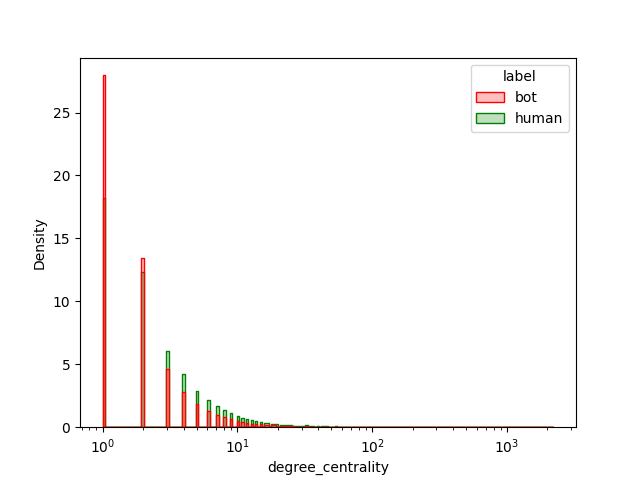
\includegraphics[width=0.75\textwidth]{complete_degree_centrality.png}
                    \caption{Degree Centrality distribution for complete network}
                \end{figure}
                \begin{figure}[H]
                    \centering
                    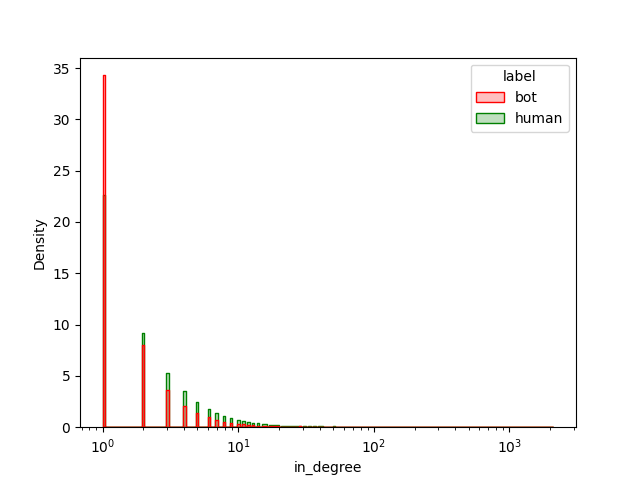
\includegraphics[width=0.75\textwidth]{complete_in_degree.png}
                    \caption{In-Degree Centrality distribution for complete network}
                \end{figure}
                \begin{figure}[H]
                    \centering
                    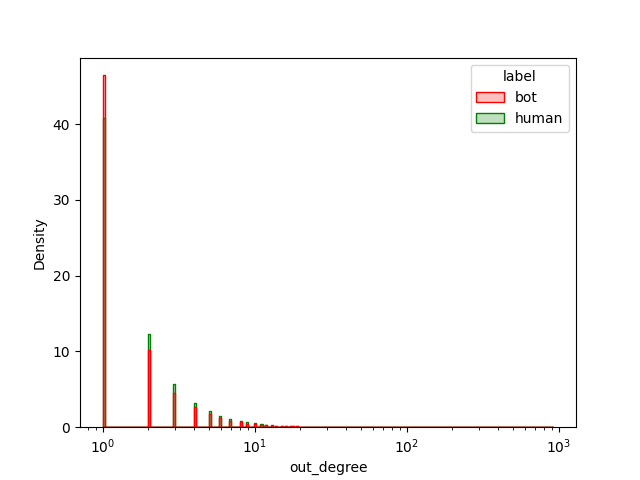
\includegraphics[width=0.75\textwidth]{complete_out_degree.png}
                    \caption{Out-Degree Centrality distribution for complete network}
                \end{figure}
			\item \textbf{Reputation.} Strictly tied to the degree centralities results are those from the reputation score, since they are derived from it.
                The obtained results match our predictions, as we can observe that the majority of humans fall in the central bins, having an average reputation score, with some notable ones having a very high score, close to 1. Concerning bots, we can instead notice a high concentration of low reputation scores. Surprisingly, there is still a quite noticeable number of bots with an average reputation score, but we can notice that there are almost no bots with very high reputation scores.
                \begin{figure}[H]
                	\centering
                    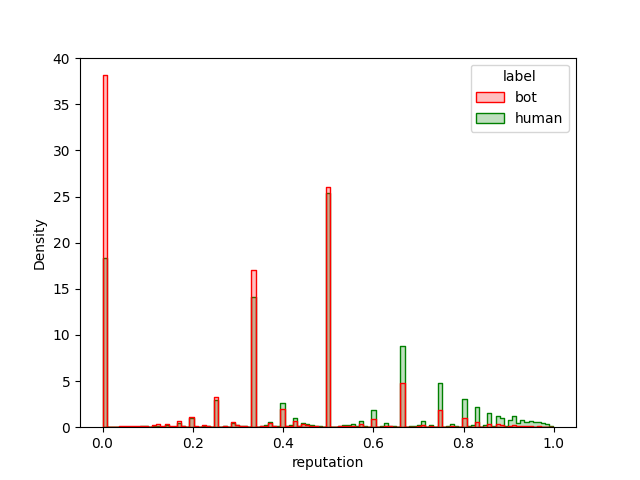
\includegraphics[width=0.75\textwidth]{complete_reputation.png}
                    \caption{Reputation distribution for complete network}
                \end{figure}
			\item \textbf{Reciprocity.} The results obtained for this measure are inconclusive. Even if our expectation was to find a bigger density of bot nodes near extreme values and a more homogeneous distribution for human users in the graphs [REFERENCE] we can observe that every distribution has his own patterns. As we expected the distributions of bots are usually skewed towards the extremes but the humans, in opposition with our beliefs, present a similar behaviour.
				\begin{figure}[H]
                	\centering
                    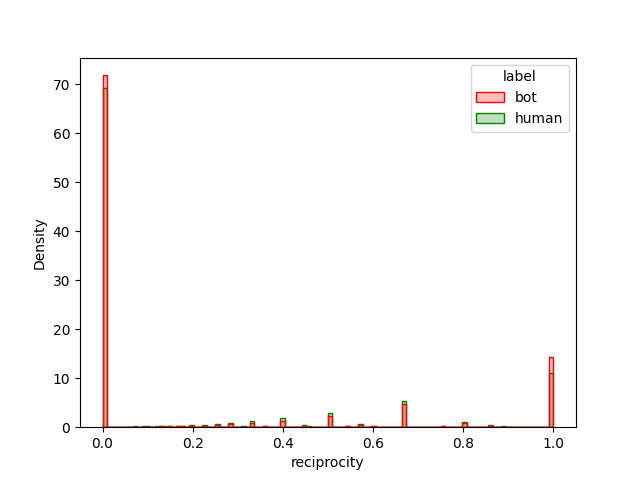
\includegraphics[width=0.75\textwidth]{complete_reciprocity.png}
                    \caption{Reciprocity distribution for complete network}
                \end{figure}
			\item \textbf{Betweenness centrality.}
                \begin{figure}[H]
                    \centering
                    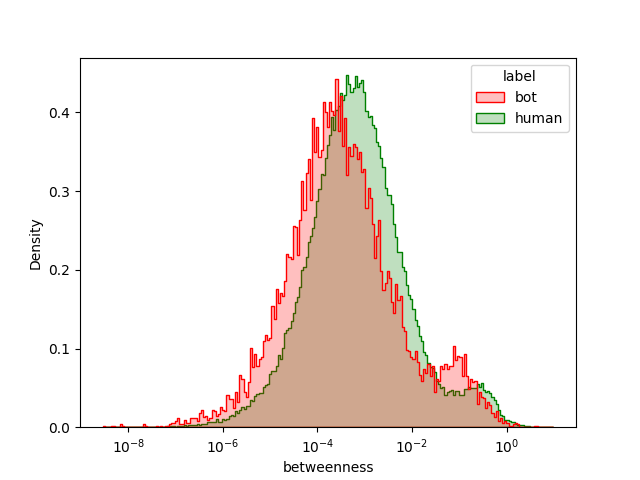
\includegraphics[width=0.75\textwidth]{complete_betweenness.png}
                    \caption{Betweenness Centrality distribution for complete network}
                \end{figure}
			\item \textbf{Eigenvector centrality.}
				\begin{figure}[H]
                    \centering
                    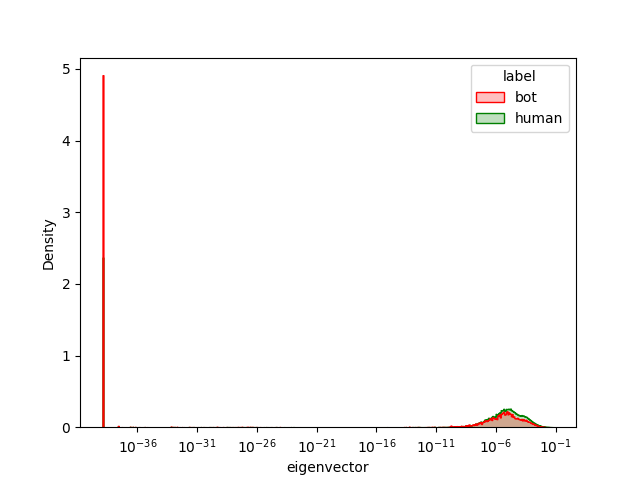
\includegraphics[width=0.75\textwidth]{complete_eigenvector.png}
                    \caption{Eigenvector Centrality distribution for complete network}
                \end{figure}      
			\item \textbf{PageRank.}
                \begin{figure}[H]
                    \centering
                    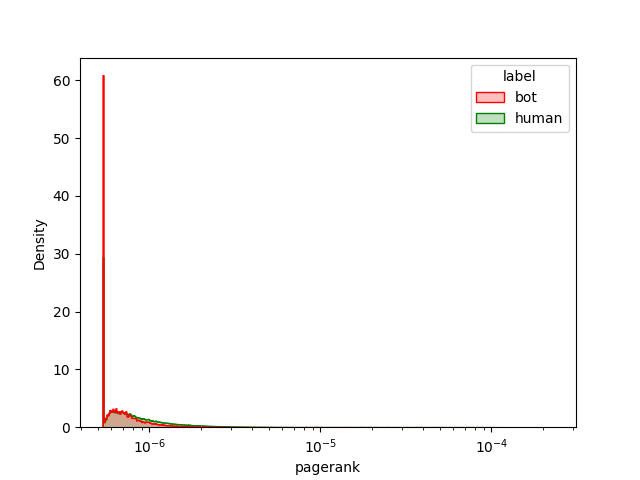
\includegraphics[width=0.75\textwidth]{complete_pagerank.png}
                    \caption{Pagerank Centrality distribution for complete network}
                \end{figure}
            \item \textbf{Hubs \& Authorities.}
                \begin{figure}[H]
                    \centering
                    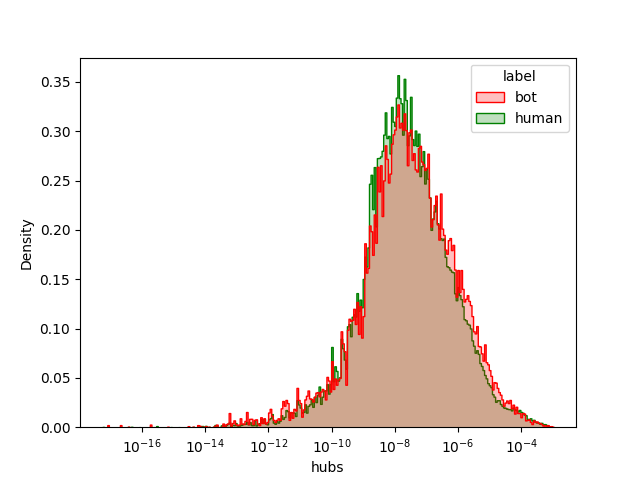
\includegraphics[width=0.75\textwidth]{complete_hubs.png}
                    \caption{Hubs scores distribution for complete network}
                \end{figure}
                \begin{figure}[H]
                    \centering
                    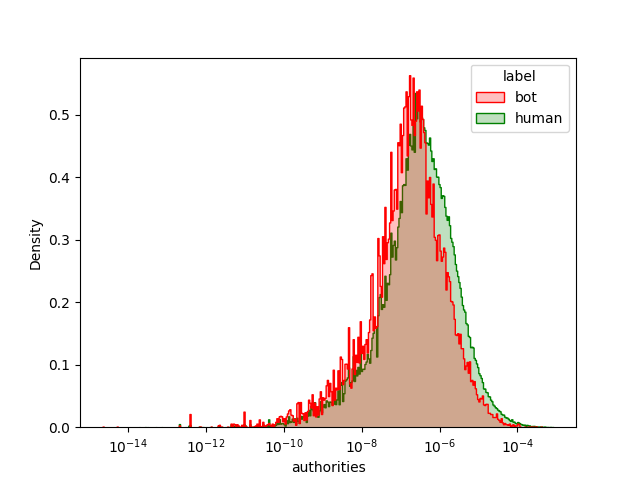
\includegraphics[width=0.75\textwidth]{complete_authorities.png}
                    \caption{Authority scores distribution for complete network}
                \end{figure}
                \begin{figure}[H]
                    \centering
                    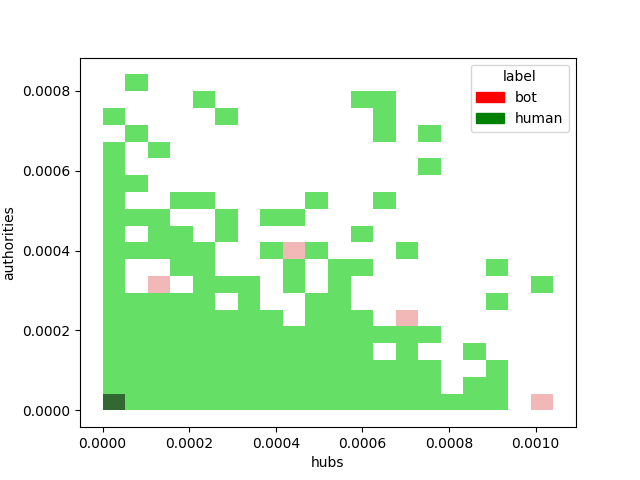
\includegraphics[width=0.75\textwidth]{complete_hubs&authorities.png}
                    \caption{Hubs and Authorities joint distribution for complete network}
                \end{figure}
		\end{itemize}
		\paragraph{Clustering Coefficient.}
        \begin{figure}[H]
            \centering
            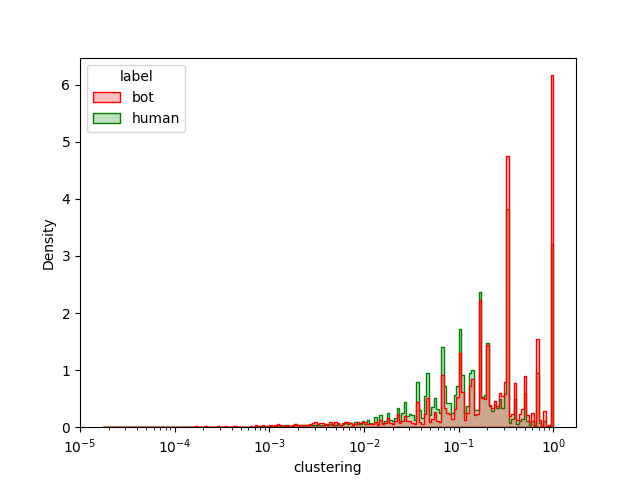
\includegraphics[width=0.75\textwidth]{complete_clustering.png}
            \caption{Clustering coefficients distribution for complete network}
        \end{figure}
		\paragraph{Average Neighbourhood Degree.}
		\begin{figure}[H]
			\centering
            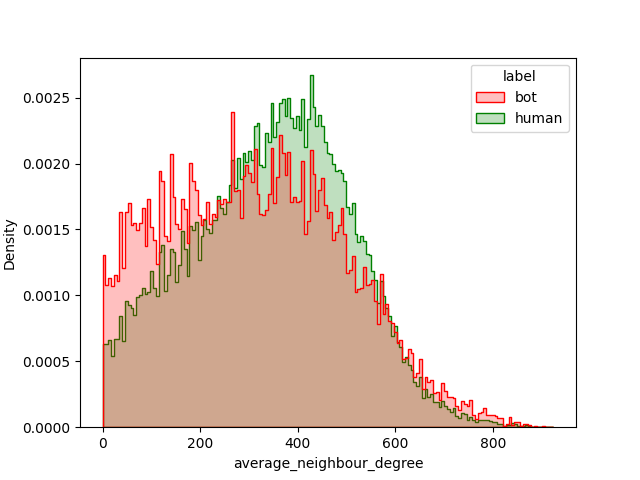
\includegraphics[width=0.75\textwidth]{complete_average_neighbour_degree.png}
            \caption{Average Neighbourhood Degree distribution for complete network}
        \end{figure}
        \paragraph{Number of Triangles.}
        \begin{figure}[H]
        	\centering
            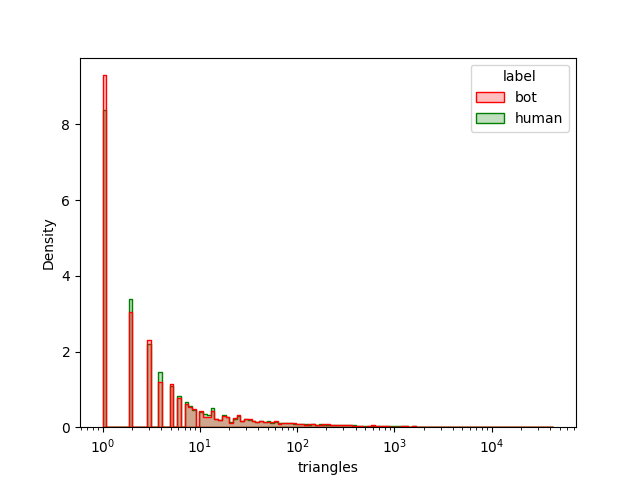
\includegraphics[width=0.75\textwidth]{complete_triangles.png}
            \caption{Number of Triangles distribution for complete network}
        \end{figure}
		\paragraph{Core Number.}
		\begin{figure}[H]
        	\centering
            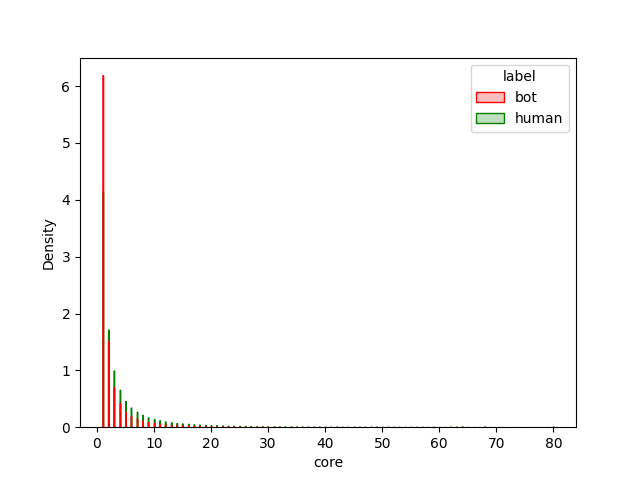
\includegraphics[width=0.75\textwidth]{complete_core.png}
            \caption{Core Number distribution for complete network}
        \end{figure}
        \paragraph{Number of Tweets.}
        \begin{figure}[H]
        	\centering
        	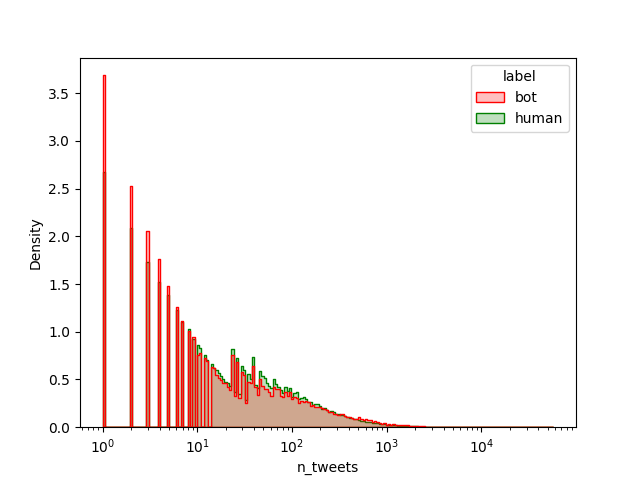
\includegraphics[width=0.75\textwidth]{complete_n_tweets.png}
            \caption{Number of Tweets distribution for complete network}
      	\end{figure}
    \subsection{Classification}
    	To discover the most reliable relationships between the extracted measures and the labels (bot and human), we decided to deploy three classical machine learning techniques for binary classification, as they would help highlight the most relevant features while ignoring the least relevant ones. This activity was also necessary since no effective trend was noticed by examining each individual distribution across all measures.\\
    	As previously stated, three approaches were attempted:
    	\begin{itemize}
        	\item Na\"ive Bayes Classifier
        	\item Random Forest Classifier
        	\item Logistic Regressor Classifier
    	\end{itemize}
    	One of the aspects we wanted to test was the capability of subnetworks of capturing aspects of the complete network, so we opted for a specialised pipeline for the training and testing.\\
    	All measures were considered for the dataset, while the labels were used to indicate the target class. First we considered all the measures obtained from one of the individual networks and used those as bases for the training and testing set, splitting them for 80\% and 20\% respectively. Each model was then trained and evaluated using the described data.\\
    	To evaluate the generalisation capabilities of each network, we extracted a random sample of 5000 users measures which were not included in the previous training and testing from the complete network. The model was then tested on those.\\
    	Lastly, after observing the results of the previous experiment, we decided to train these models, which were picked for their capability of handling large quantities of data, on the entire dataset. After an 80/20 train/test split on the measures of the full graph, we proceeded with training and evaluation.
    	To evaluated the results themselves we computed the accuracy and the F1 score of each prediction, producing a confusion matrix for better visualisation.
    \subsection{Classification discussion}
		

\section{Conclusion}
	\label{conclusion}
	% Qualitative analysis of the quantitative findings of the study.
    

\section{Critique}
	\label{critique}
	% Do you think your work solves the problem presented above? To which extent (completely, what parts)? Why? What could you have done differently to answer your research problems (e.g., gather data with additional information, build your model differently, apply alternative measures)?
	The \textit{follower} and \textit{following} connections may not represent meaningful relations for bot detection, as the TwiBot-22 dataset lacks a clear separation between human and bot accounts in this aspect.


\newpage
\bibliographystyle{plain}
\bibliography{references}

\end{document}
